\chapter{A/B testing}
\label{ch-a-b-testing}

{\bf A/B testing} in its simplest
form is just frequentist {\bf hypothesis testing (HT)}.
The formulae used for HT
will not be  derived here. 
In this chapter, we will merely state them,
and draw a causal bnet describing them.


\begin{figure}[h!]

{\entrymodifiers={++[F-:<3pt>]}

$$\xymatrix@R=25pt{
\alp\ar@/_2pc/[dd]\ar[d]
&
\beta\ar[d]
&
\vv{p}\ar@/_2pc/[dd]
\ar[dr]
\ar[d]
\ar[ddr]
&\vv{n}\ar[d]
\\
Z_{\alp/2}\ar[drr]
\ar[drrr]
&Z_\beta\ar[dr]
&Z\ar[dl]
&\vv{SE}\ar[l]\ar[d]
\\
\text{decision}
&p\ar[l]
&n
&CI
}$$
}
\caption{Bnet for A/B testing (a.k.a. 
hypothesis testing.)}
\label{fig-bnet-hypo-test}
\end{figure}

Fig.\ref{fig-bnet-hypo-test}
gives a bnet for HT. The node names 
of the bnet are defined as follows

$\Phi()$: Cumulative Distribution
of Standard Normal Distribution
\beq
\Phi (x)=\frac{1}{\sqrt{2\pi}}
\int_{-\infty}^x dt\; e^{
-\frac{t^2}{2}}
\eeq

Conversions: The number of successful actions (e.g., purchases, sign-ups). 

$\xi\in\{A,B\}$: Variant. A is the control group
and the null Hypothesis $H_0$, B is 
the treated group
and the alternative hypothesis $H_1$.
 
$p_\xi$: Conversion rate, the proportion of users who converted (for variant $\xi$).

$\vv{p}=(p_A, p_B)$

$n_\xi$: Sample size, number of visitors
(for variant $\xi$).
   
$\vv{n}=(n_A, n_B)$.

$(\alp, \beta)$: tail areas. One minus tail area = confidence level. $\alp=P(0|1)=$ probability of type 1 error. $\beta=P(1|0)=$
probability of type 2 error. See Table
\ref{tab-ht-terms}.

% Please add the following required packages to your document preamble:
% \usepackage[table,xcdraw]{xcolor}
% Beamer presentation requires \usepackage{colortbl} instead of \usepackage[table,xcdraw]{xcolor}
\begin{table}[h!]
\begin{tabular}{|l|l|l|}
\hline
 & \cellcolor[HTML]{FFFFC7}0 actual & \cellcolor[HTML]{FFFFC7}1 actual \\ \hline
\cellcolor[HTML]{FFFFC7}0 predicted & \begin{tabular}[c]{@{}l@{}}$P(0|0)$\\ True Negative\end{tabular} & \begin{tabular}[c]{@{}l@{}}$P(0|1)$\\ $\beta$\\ Type II error\\ False Negative\end{tabular} \\ \hline
\cellcolor[HTML]{FFFFC7}1 predicted & \begin{tabular}[c]{@{}l@{}}$P(1|0)$\\ $\alp$\\ Type I error\\ False Positive\end{tabular} & \begin{tabular}[c]{@{}l@{}}$P(1|1)$\\ True Positive\end{tabular} \\ \hline
\end{tabular}
\caption{Terminology associated with hypothesis testing}
\label{tab-ht-terms}
\end{table}
$SE_\xi$: Standard error, measuring the variability of the conversion rate
(for variant $\xi$).
Called $\s_\xi/\sqrt{n_\xi}$ in Statistics.
    
$\vv{SE}=(SE_A, SE_B)$

$Z_\alp$: Z-score for
tail area $\alp$. Confidence level
 $CL_\alp=1-\alp$ (e.g., $Z=1.96$ for $CL=95$\%).  

$Z_\beta$: Z-score for tail area $\beta$




$n$: Minimum required sample size.
We require $n_A, n_B\geq n$.

$CI$: Confidence interval.  

$Z$: Z-score, measuring how different the two conversion rates are in standard deviation units.

$p$: p-value

decision: whether the result is statistically significant or not.

The structure equations of the nodes
of the bnet are defined as follows:


\begin{enumerate}

\item {\bf Confidence Levels (CL)}

\beq
CL_\alp = 1-\alp\;,\;\; CL_\beta = 1-\beta
\eeq

This applies to both one-tailed and two-tailed testing.


\item {\bf Conversion Rate (a.k.a., proportion)(p)}  

\beq
p_\xi = \frac{\text{Conversions for $\xi$}}{\text{Total Visitors for $\xi$}}
\eeq
for $\xi=A,B$.

\item {\bf Standard Error (SE)}  

\beq
SE_\xi = \sqrt{\frac{p_\xi  (1 - p_\xi)}{n_\xi}}
\eeq
for $\xi=A,B$.


\item {\bf Z-Score (for hypothesis testing)}  

\beq
Z = \frac{p_A - p_B}{\sqrt{SE_A^2 + SE_B^2}}
\eeq

\item {\bf P-Value}  

\beq
p=
\left\{
\begin{array}{ll}
1 -\Phi(|Z|)
&\text{if one-tail testing}
\\
2[1 -\Phi(|Z|)]
&\text{if two-tailed testing }
\end{array}
\right.
\eeq
See Fig.\ref{fig-p-def-a-b}.

\begin{figure}[h!]
\centering
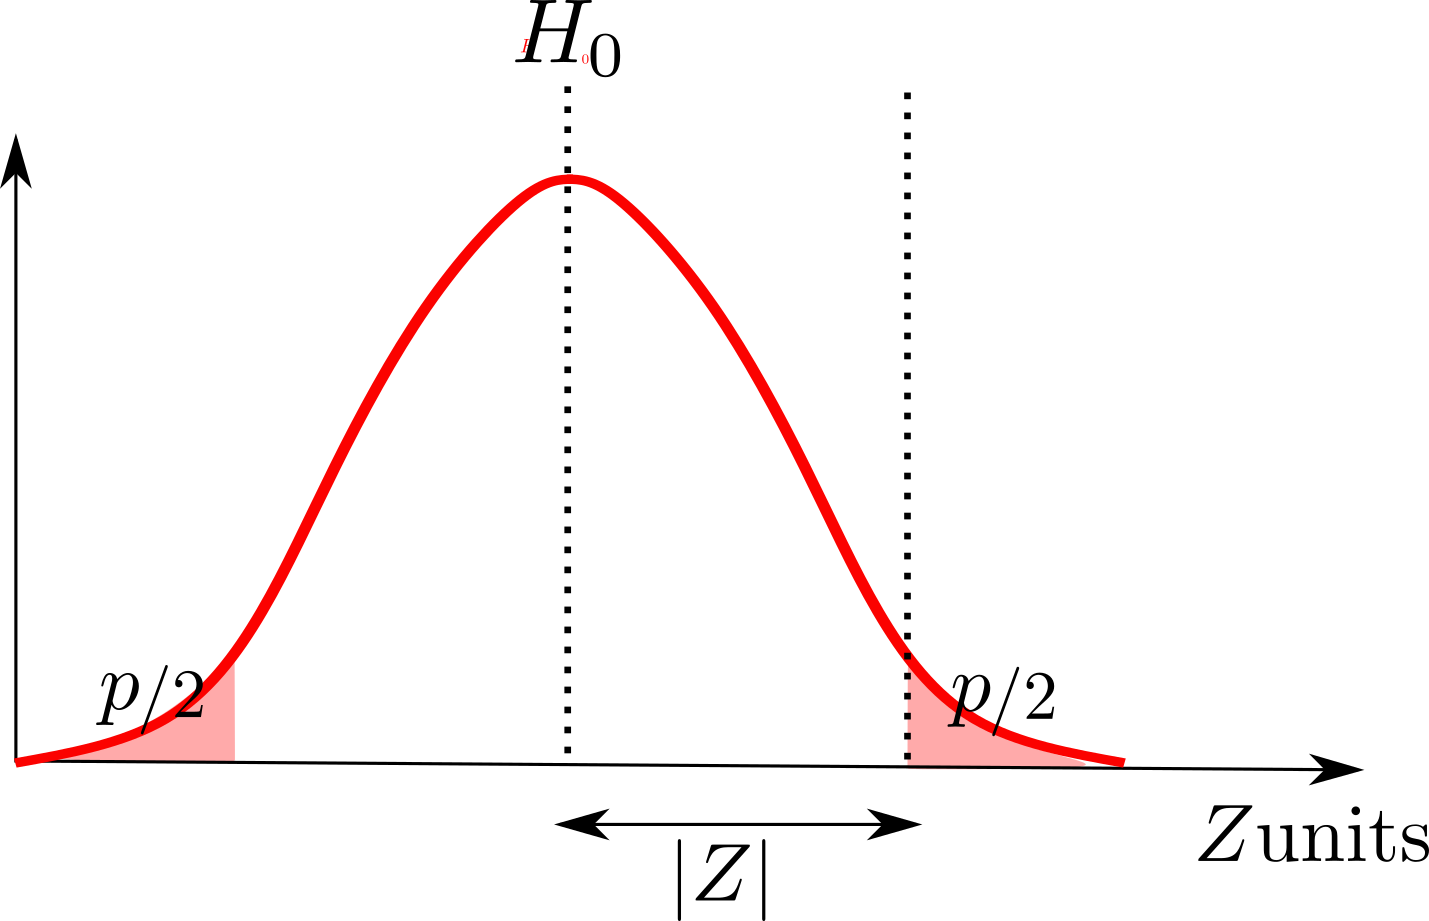
\includegraphics[width=2.5in]
{a-b-testing/p-def.png}
\caption{How $Z$ is
related to $p/2$.}
\label{fig-p-def-a-b}
\end{figure}



\item {\bf Decision}

Say $\alp=0.05$ (95\% confidence level)

If $p< \alp$,  overlap between Gaussians is small, reject null hypothesis,
a statistically significant result

If $p \geq \alp$, overlap between Gaussians is large, fail to reject null hypothesis, not a statistically significant result

\item {\bf $Z_\alp, Z_\beta$  scores}

\beq
Z_\alp=
\Phi^{-1}(1 -\alp)
\eeq
Same with $\alp$ replaced by $\beta$.
Use $Z_{\alp/2}$ for two-tailed testing, $Z_\alp$ for one-tailed testing. See Fig.\ref{fig-alp-beta-z}.

\begin{figure}[h!]
\centering
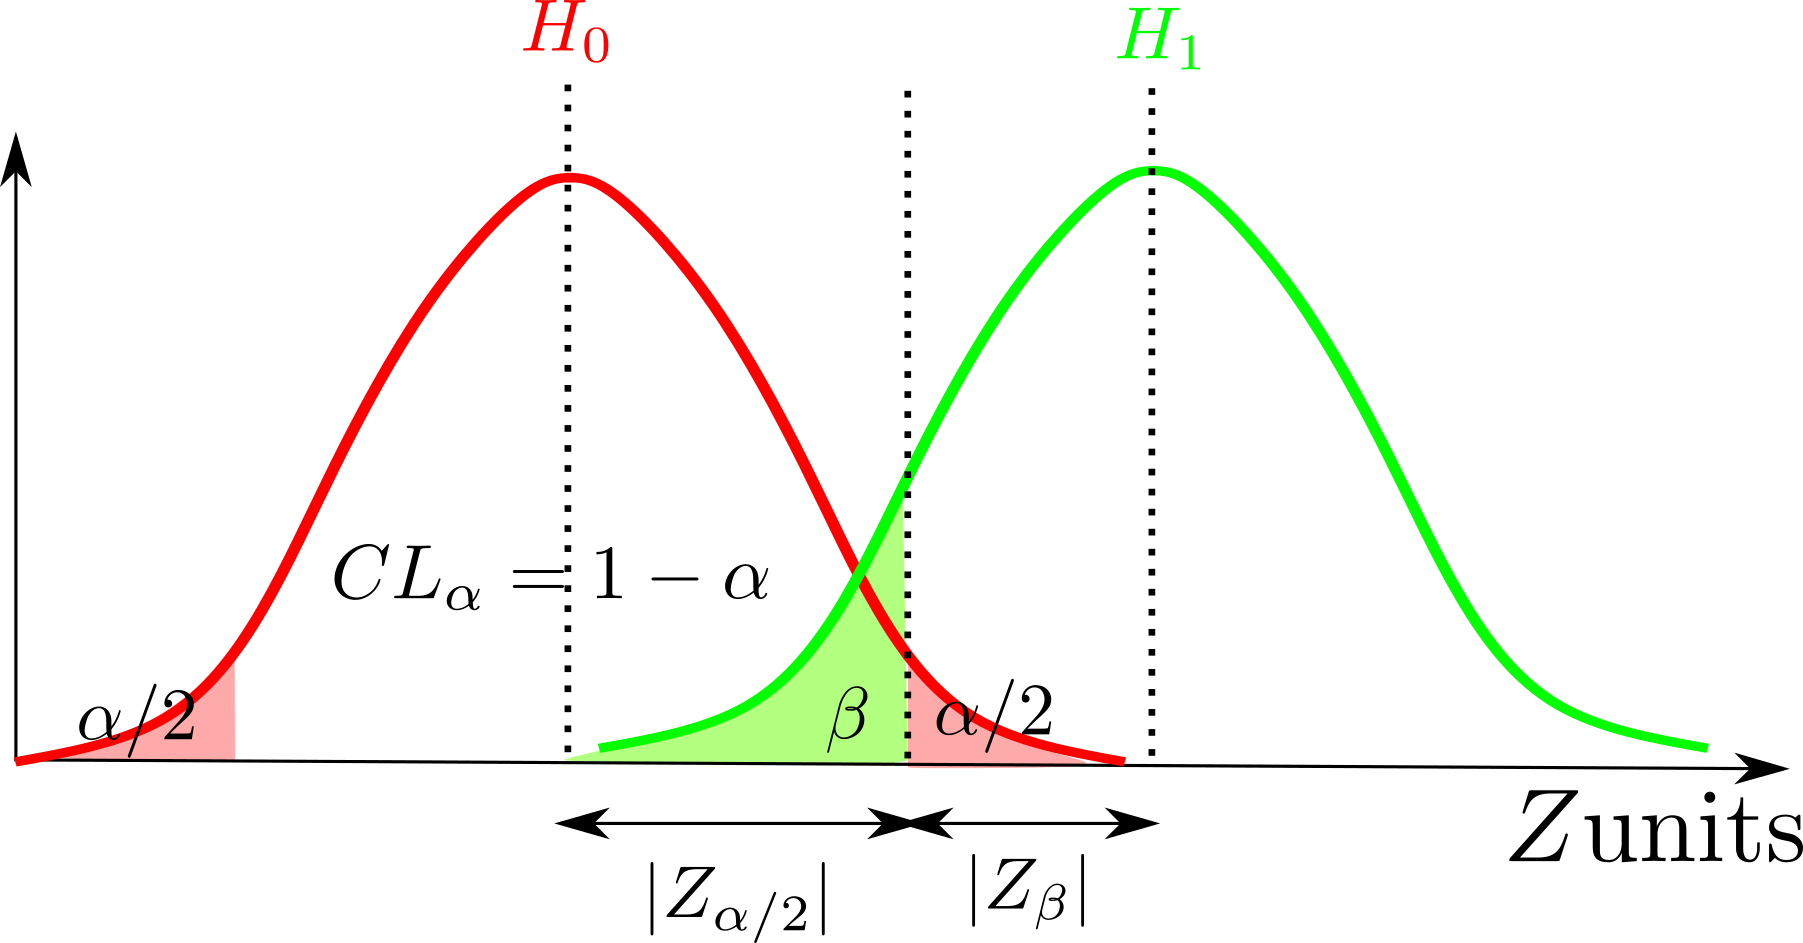
\includegraphics[width=3.5in]
{a-b-testing/alp-beta-z.png}
\caption{How $Z_{\alp/2}$ and $Z_\beta$ are
related to $\alp/2$ and $\beta$.}
\label{fig-alp-beta-z}
\end{figure}

\item {\bf Confidence Interval for Difference in Proportions} 

\beq
a_\pm = (p_A - p_B) \pm Z_{\alpha/2} \sqrt{SE_A^2 + SE_B^2}
\eeq

\beq
CI = [a_-, a_+]
\eeq



\item {\bf Sample Size 
(for Proportion Tests)}
\beq
n = 
\left[
\frac{
Z_{\alpha/2}
\sqrt{2p_A(1-p_A)}
+Z_\beta 
\sqrt{p_A(1-p_A) + p_B(1-p_B)}
}{p_A - p_B}
\right]^2
\eeq
We require $n_A, n_B\geq n$.
At first, $p_A$ is known, but $p_B$ 
must be
estimated because it is unknown.
\end{enumerate}
